\section{Frontend Implementierung}
\setauthor{Jonas Dorfinger}

Die Anforderungen an das Frontend sind sehr vielseitig, einerseits soll es wie eine Präsentation mit mehreren Slides aufgebaut,
andererseits soll das gesamte Projekt leicht wartbar und individualisierbar bleiben.
Die Daten werden dynamisch aus einem Konfigurationsfile ausgelesen, welches durch einen eigenen Generator generiert werden kann.

Um die UserExperience zu verbessern, wird auch auf wichtigen Dinge wie Angular Routing oder angemessenes styling Wert gelegt.
Nicht zu vernachlässigen ist dabei, der Fakt, dass webmap interaktiv sein soll.
Das bedeutet, dass der Userin oder dem User die Möglichkeit geboten werden soll, durch Slider oder true/false Switches
die Darstellung der aktuellen Daten auf der Page zu manipulieren.


\cleardoublepage

\subsection{Konfigurationsfile}
Das Konfigurationsfile ist ein JSON File, welches festlegt welche Slides (Pages) existieren, aber auch die zu darstellenden Daten definiert.
Hinweis: Grafische Darstellungen der Konfiguration sind weiter unten, bei anderen Kapiteln angeführt.

\begin{lstlisting}[label={lst:config.json}]{config.json}
{
  "name": "webmap showcase",
  "description": "this config is made to show how webmap configs look like",
  "pages": [
    {
      "title": "Bersbuch",
      "subtitle": "Anreise Dauer zum Bahnhof Bersbuch.",
      "description": [
        "Bersbuch ist ein Dorf in der Gemeinde Andelsbuch im Bregenzerwald."
      ],
      "mapOptions": {
        "zoom": 13,
        "center": [
          47.40198749647868,
          9.861946105957031
        ]
      },
      "datasources": [
        {
          "options": {},
          "id": "bersbuch-walk"
        }
      ],
      "controls": {
        "filters": [
          {
            "name": "Anreise Dauer Rad",
            "type": "slider",
            "dataSource": "bersbuch-bike",
            "unit": "Sekunden",
            "filterValue": "time"
          }
        ]
      }
    }
  ],
  "datasources": [
    {
      "options": {},
      "data": "bersbuch_walk.json",
      "id": "bersbuch_walk",
      "colorScheme": "my-color-scheme",
      "colorSchemeOrderValue": "time",
      "tooltip": [
        {
          "type": "value",
          "name": "time"
        },
        {
          "type": "text",
          "content": " Sekunden"
        }
      ]
    }
  ],
  "customColorSchemes": [
    {
      "id": "my-color-scheme",
      "colors": [
        "#f6d2a9",
        "#f5b78e",
        "#f19c7c",
        "#ea8171",
        "#dd686c",
        "#ca5268",
        "#b13f64"
      ]
    }
  ]
}
\end{lstlisting}

\subsubsection{Allgemeine Properties}
\textbf{Name}
Verleiht der ganzen Seite einen Namen.
Wird aktuell nicht angezeigt, kann aber durch Individualisierungen verwendet werden.

\textbf{Description}
Beschreibt die erzeugte Website etwas genauer.
Wird aktuell nicht angezeigt, kann aber durch Individualisierungen verwendet werden.

\subsubsection{Pages}
\emph{Pages} ist ein Array, welches die Ansichten definiert.
Jedes Element im Array, hat eine eigenen Map Ansicht, sowie eigene Daten, welche in der Sidebar angezeigt werden.

\textbf{Title}
ist der Name der Seite und wird groß hervorgehoben angezeigt.

\textbf{Subtitle}
Der Subtitle beschreibt in wenigen Wörtern, etwas genauer worum es bei der ausgewählten Karte geht.

\textbf{Description}
Description ist in diesem Fall ein Array von Strings, das bedeutet, es können mehrere Texteinträge angeführt werden,
was wiederrum einen Designtechnischen Grund hat.
Für jeden Eintrag wird ein eigener Absatz in der Sidebar generiert.

\textbf{Map Options}
Hier können in einem freien JSON Feld \href{https://leafletjs.com/SlavaUkraini/reference.html#map-option}{Leaflet-Map-Options}
übergeben werden, um die Darstellung der Map gezielt zu verändern.
Ein häufiger Anwendungsfall dafür ist es, den Ausrichtungspunkt zu ändern, um automatisch den richtigen Kartenausschnitt präsentiert zu bekommen.

\textbf{Data Sources}
Bei dem Array \emph{Data Sources} können Geo-Daten eingebunden werden, weiter unten werden diese Global definiert und hier
können diese referenziert werden.
Zusätzlich können wieder \emph{options}, in Form von einem JSON Objekt übergeben werden.

\textbf{Controls}
Hier können interaktive Elemente ausgewählt werden.
Es gibt vordefinierte Controls, aus denen man wählen kann.
Nach Absprache mit der triply, wurde entschieden, dass für diese Version ein Filter ausreichend ist.
Dieser Filter ist ein Slider, welcher auf eine bestimmte Property gebindet werden kann (\emph{filterValue}).
Mit dem Attribut \emph{dataSource} wird die zutreffende Data Source ausgewählt.
Zusätzlich kann noch eine Einheit (\emph{unit}) und auch ein Name für den Filter angegeben werden.

\subsubsection{Data Sources}
Ist ein Array
%TODO schreib den gack

\textbf{ID}
Die ID wird benötigt, um eine Data Source referenzieren zu können, zum Beispiel bei der Erstellung von Pages.

\textbf{Data}
Data ist ein File-upload Feld, bei dem kann das Geo-JSON File hochgeladen werden, in welchem die Daten gespeichert sind.

\textbf{Options}
Hier können \href{https://leafletjs.com/SlavaUkraini/reference.html#map-option}{Leaflet-Map-Options} in einem freien JSON-Feld
übergeben werden, um die Art der Darstellung oder das Verhalten der Map zu verändern.

\textbf{Color Scheme}
Dieses Feld referenziert auf die ID eines Color Schemes, entweder man gibt den Namen eines
\href{https://carto.com/carto-colors/}{Carto-Color-Schemes} an oder man erstellt ein eigenes Custom-Color-Scheme.

\textbf{Color Scheme Order Value}
Um das Color-Scheme richtig anzuwenden, braucht man einen Value, um eine angemessene Skalierung zu berechnen, dieser Attributname
kann hier angegeben werden.

\textbf{Tooltip}
Der Tooltip ist ein Feature, welcher es ermöglicht Information beim hovern einer Data Source auf der Map anzuzeigen.
Es ist deshalb ein Array, damit man unbegrenzt viele Informationen angeben kann.
Jedes JSON-Objekt in diesem Array besitzt genau 2 Attribute, \emph{type} und \emph{name} oder \emph{content}.
Der \emph{type} gibt an, ob es sich um einen Value oder einen Text handelt, bei einem Value, muss der Attributname, des
Values bei dem anderen Attribute (\emph{Name}) angegeben werden.
Wird jedoch der Typ \emph{Text} ausgewählt, so muss lediglich ein String angegeben werden, welcher angezeigt wird (zum Beispiel
eine Einheit für den Value zuvor).

\subsubsection{Custom Color Schemes}
Hierbei handelt es sich um ein Array, in dem individuelle Color Schemes gespeichert werden können.
Wichtig, dass auch hier jedes JSON-Objekt eine ID erhält, um das Scheme referenzieren zu können.
Weiters befindet sich ein Array \emph{colors} in diesem Objekt, welches die HEX-Codes der Farben beinhaltet.

\subsection{Sidebar}

\subsection{Mapview}

\subsection{Global Datasources}

\subsection{Custom Color Schemes}

\subsection{Navigation}

\begin{figure}[hbt!]
    \centering
    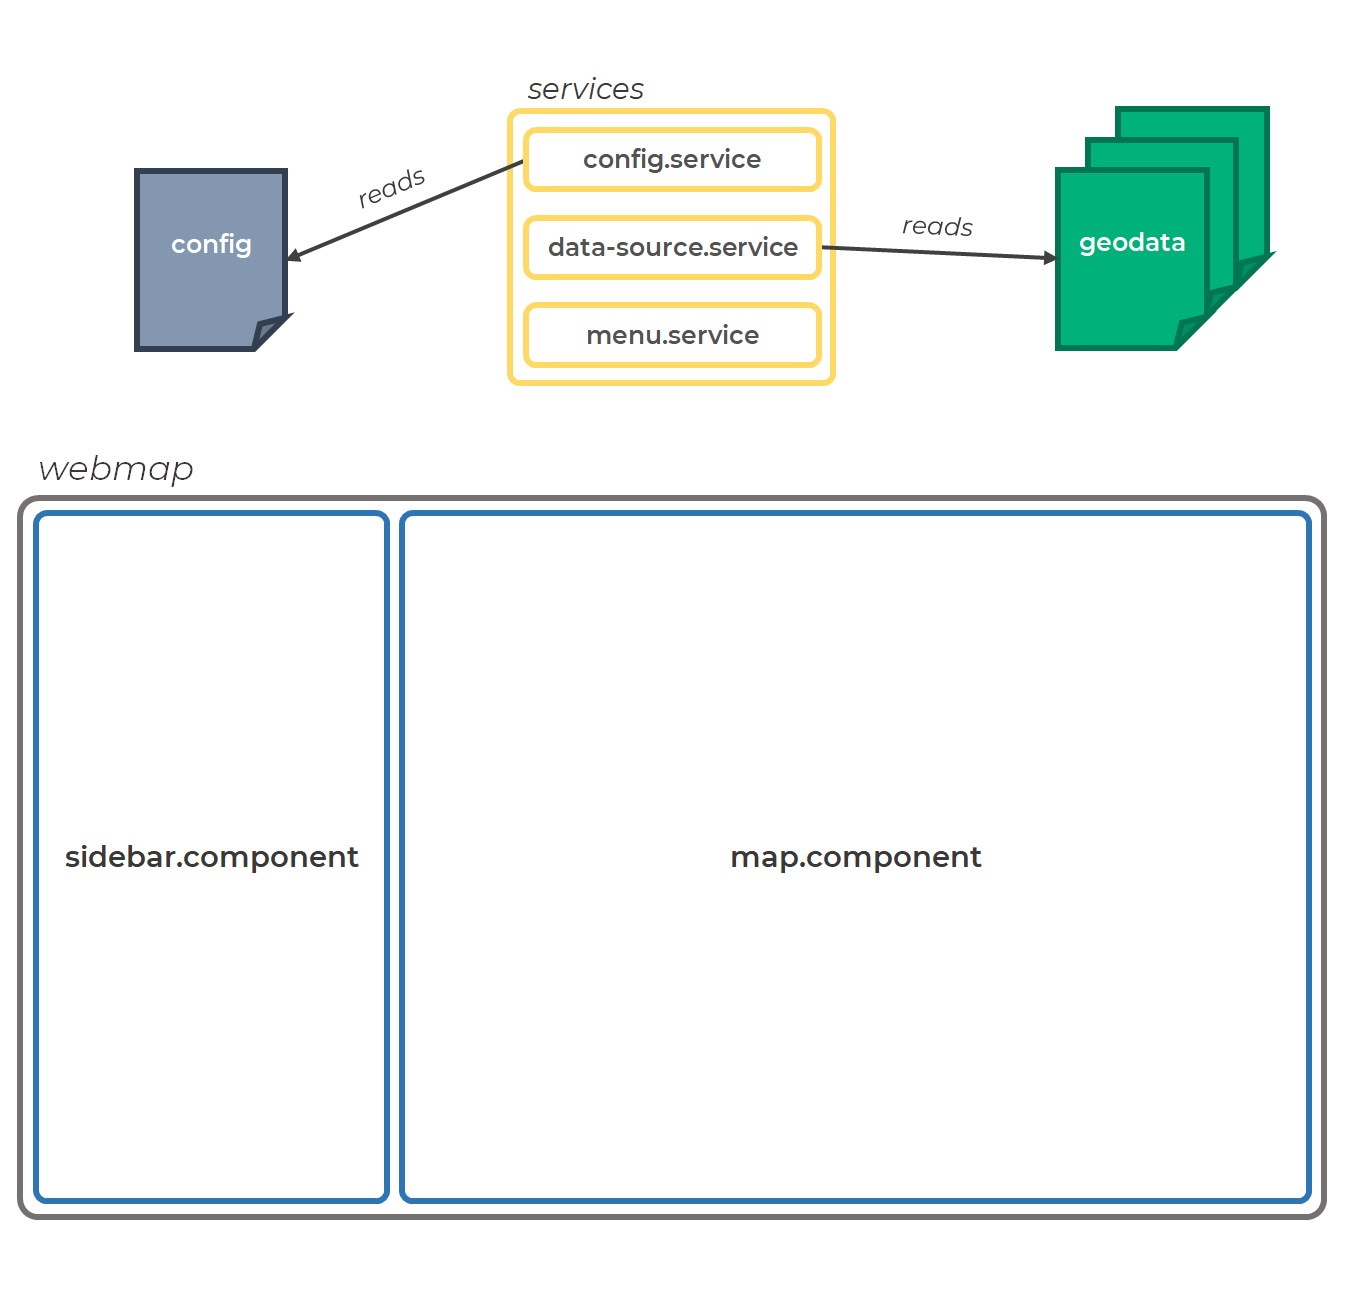
\includegraphics[scale=.6]{pics/frontend-architecture}
    \caption{Frontend Architektur}
    \label{fig:frontend-architecture}
\end{figure}